\documentclass[border=2pt]{standalone}
\usepackage[utf8]{inputenc} % Required for inserting images
\usepackage{tikz}
\usepackage{helvet}
\usetikzlibrary{shapes.geometric, arrows}
\pagecolor{white}

%-------------------------defining colorblind friendly colors
% Using pale color scheme in Figure 6 
% by Paul Tol https://personal.sron.nl/~pault/
\definecolor{cbblue}{HTML}{BBCCEE}
\definecolor{cbcyan}{HTML}{CCEEFF}
\definecolor{cbgreen}{HTML}{CCDDAA}
\definecolor{cbyellow}{HTML}{EEEEBB}
\definecolor{cbred}{HTML}{FFCCCC}
\definecolor{cbgrey}{HTML}{DDDDDD}

% -------------------------defining nodes 
\tikzstyle{input} = [trapezium, trapezium left angle =80, trapezium right angle = 100,
minimum width= 3cm, minimum height=0.5cm, text centered, draw=black, fill=cbblue]
\tikzstyle{process} = [rectangle, minimum width = 3cm, minimum height = 1cm,
text centered, , text width=4cm,draw=black, fill=cbgrey]
\tikzstyle{decision} = [diamond, minimum width = 3cm, minimum height = 1cm,
text centered, , text width=3.5cm, draw=black, fill=cbcyan]
\tikzstyle{changeclass} = [rectangle, rounded corners, minimum width=3cm, minimum height=1cm,
text centered, draw = black, fill=cbyellow]
\tikzstyle{reject} = [trapezium, trapezium left angle =80, trapezium right angle = 100,
minimum width= 1cm, minimum height=0.5cm, text centered, draw=black, fill=cbred]
\tikzstyle{accept} = [trapezium, trapezium left angle =80, trapezium right angle = 100,
minimum width= 1cm, minimum height=0.5cm, text centered, draw=black, fill=cbgreen]

% -------------------------defining connectors
\tikzstyle{arrow} = [thick,->, >=stealth]
\tikzstyle{line} = [thick,-,>=stealth]
\begin{document}

% ------------------------- tikz image (flow chart)
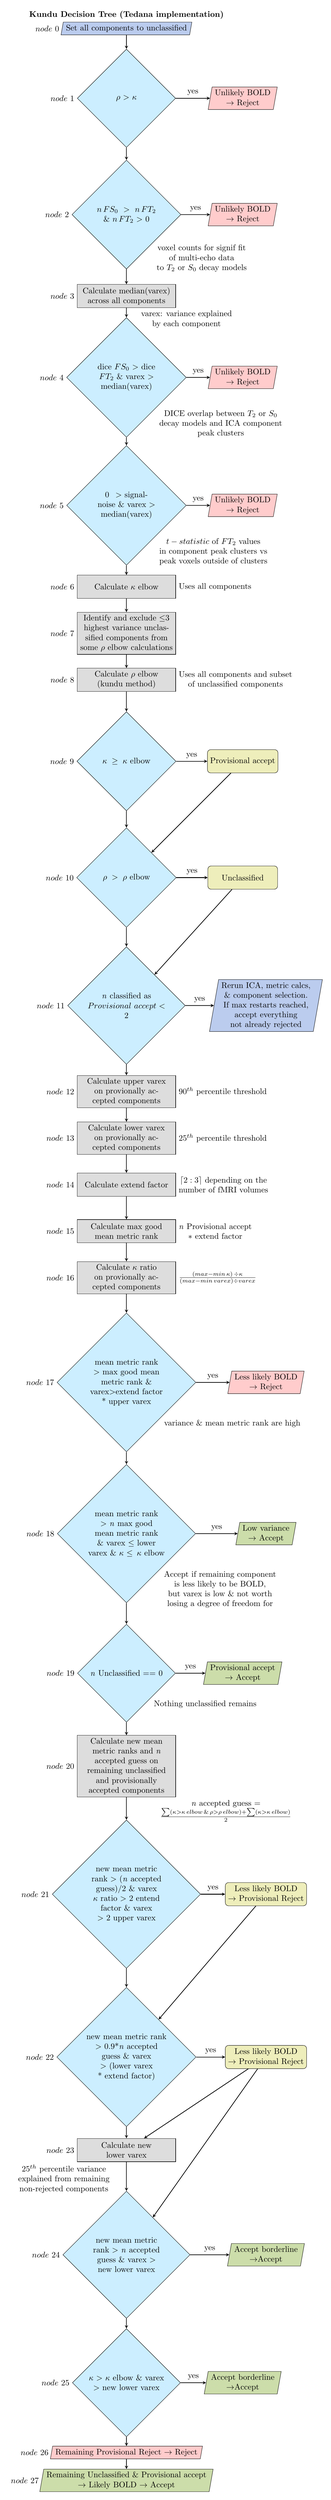
\begin{tikzpicture}[node distance = 2cm]

% ------------------------- nodes -------------------------

% ----- node: 0
\node(0)[input, label={90:\textbf{Kundu Decision Tree (Tedana implementation)}}, label={180:$node\ 0$}] {Set all components to unclassified};
% ----- node: 1
\node(1)[decision, below of=0,label={180:$node\ 1$}, yshift=-1.0cm]{$\rho$ $>$ $\kappa$};
\node(rej0)[reject, right of=1, xshift=3cm, align=center]{Unlikely BOLD\\$\rightarrow$ Reject};
% ----- node: 2
\node(2)[decision, below of=1,label={180:$node\ 2$} ,label={[align=center] 315: voxel counts for signif fit\\of multi-echo data\\to $T_2$ or $S_0$ decay models}, yshift=-3.0cm]{$n \, FS_0 \, > \, n \, FT_2$ \& $n \,FT_2$ $>$ 0};
\node(rej1)[reject, right of=2, xshift=3cm, align=center]{Unlikely BOLD\\$\rightarrow$ Reject};
% ----- node: 3
\node(3)[process, below of=2, label={180:$node\ 3$}, label={[align=center] 315: varex: variance explained\\by each component}, yshift=-1.5cm]{Calculate median(varex) across all components};
% ----- node: 4
\node(4)[decision, below of=3,label={180:$node\ 4$},label={[align=center] 315:DICE overlap between $T_2$ or $S_0$\\decay models and ICA component\\peak clusters}, yshift=-1.5cm]{dice $FS_0$ $>$ dice $FT_2$ \& varex $>$ median(varex)
};
\node(rej2)[reject, right of=4, xshift=3cm, align=center]{Unlikely BOLD\\$\rightarrow$ Reject};
% ----- node: 5
\node(5)[decision, below of=4,label={180:$node\ 5$}, label={[align=center] 315: $t-statistic$ of $FT_2$ values\\in component peak clusters vs\\peak voxels outside of clusters}, yshift=-3.5cm]{ $0 \, >$ signal-noise \&  varex $>$ median(varex)};
\node(rej3)[reject, right of=5, xshift=3cm, align=center]{Unlikely BOLD\\$\rightarrow$ Reject};
% ----- node: 6
\node(6)[process, below of=5, label={180:$node\ 6$}, label={0: Uses all components}, yshift=-1.5cm]{Calculate $\kappa$ elbow};
% ----- node: 7
\node(7)[process, below of=6, label={180:$node\ 7$}, yshift=-0.0cm]{Identify and exclude $\leq$3 highest variance unclassified components from some $\rho$ elbow calculations};
% ----- node: 8
\node(8)[process, below of=7, label={180:$node\ 8$}, label={[align=center] 0: Uses all components and subset\\of unclassified components}]{Calculate $\rho$ elbow\\(kundu method)};
% ----- node: 9
\node(9)[decision, below of=8,label={180:$node\ 9$}, yshift=-1.5cm]{$\kappa \geq \kappa$ elbow};
\node(rej4)[changeclass, right of=9, xshift=3cm]{Provisional accept};
% ----- node: 10
\node(10)[decision, below of=9,label={180:$node\ 10$}, yshift=-3.0cm]{$\rho > \rho$ elbow  };
\node(rej5)[changeclass, right of=10, xshift=3cm]{Unclassified};
% ----- node: 11
\node(11)[decision, below of=10, label={180:$node\ 11$}, yshift=-3.5cm]{ \textit{n} classified as $Provisional\ accept < 2$};
\node(rej6)[input, right of=11, xshift=4cm, align=center]{Rerun ICA, metric calcs,\\\& component selection.\\If max restarts reached,\\accept everything\\not already rejected};
% ----- node: 12
\node(12)[process, below of=11,label={180:$node\ 12$},label={0: $90^{th}$ percentile threshold}, yshift=-1.7cm]{Calculate upper varex on provionally accepted components};
% ----- node: 13
\node(13)[process, below of=12,label={180:$node\ 13$}, label={0: $25^{th}$ percentile threshold},]{Calculate lower varex on provionally accepted components};
% ----- node: 14
\node(14)[process, below of=13,label={180:$node\ 14$}, label={[align=center] 0:$\lceil 2:3 \rceil$ depending on the\\number of fMRI volumes}]{Calculate extend factor};
% ----- node: 15
\node(15)[process, below of=14,label={180:$node\ 15$},label={[align=center] 0: \textit{n} Provisional accept\\$*$ extend factor}]{Calculate max good mean metric rank};
% ----- node: 16
\node(16)[process, below of=15, label={180:$node\ 16$}, label={[align=center] 0: $\frac{(max-min \, \kappa) \, \div \kappa}{(max-min \, varex) \div varex}$}]{Calculate $\kappa$ ratio on provionally accepted components};
% ----- node: 17
\node(17)[decision, below of=16,label={180:$node\ 17$},label={315:variance \& mean metric rank are high}, yshift=-2.5cm]{mean metric rank $>$ max good mean metric rank \& varex$>$extend factor * upper varex};
\node(rej7)[reject, right of=17, xshift=4cm, align=center]{Less likely BOLD\\$\rightarrow$ Reject};
% ----- node: 18
\node(18)[decision, below of=17,label={180:$node\ 18$},label={[align=center] 315: Accept if remaining component\\is less likely to be BOLD,\\but varex is low \& not worth\\losing a degree of freedom for}, yshift=-4.5cm]{mean metric rank $>$ \textit{n} max good mean metric rank \& varex $\leq$ lower varex \& $\kappa$ $\leq \, \kappa$ elbow };
\node(rej8)[accept, right of=18, xshift=4cm, align=center]{Low variance\\$\rightarrow$ Accept};
% ----- node: 19
\node(19)[decision, below of=18,label={180:$node\ 19$},label={315: Nothing unclassified remains}, yshift=-4.0cm]{\textit{n} Unclassified $==0$};
\node(rej9)[accept, right of=19, xshift=3cm, align=center]{Provisional accept\\$\rightarrow$ Accept};
% ----- node: 20
\node(20)[process, below of=19, label={180:$node\ 20$},yshift=-2.0cm, label={[align=center] 315: \textit{n} accepted guess =\\$\frac{\sum(\kappa > \kappa\, elbow\, \&\, \rho > \rho\, elbow)+ \sum(\kappa > \kappa\, elbow)}{2}$}]{Calculate new mean metric ranks and \textit{n} accepted guess on remaining unclassified and provisionally accepted components};
% ----- node: 21
\node(21)[decision, below of=20,label={180:$node\ 21$}, yshift=-3.5cm]{new mean metric rank $>$ (\textit{n} accepted guess)/2 \& varex $\kappa$ ratio $>$ 2 entend factor \& varex $>$ 2 upper varex};
\node(rej10)[changeclass, right of=21, xshift=4cm, align=center]{Less likely BOLD\\$\rightarrow$ Provisional Reject};
% ----- node: 22
\node(22)[decision, below of=21,label={180:$node\ 22$}, yshift=-5cm]{new mean metric rank $>$ 0.9*\textit{n} accepted guess \& varex $>$  (lower varex * extend factor)};
\node(rej11)[changeclass, right of=22, xshift=4cm, align=center]{Less likely BOLD\\$\rightarrow$ Provisional Reject};
% ----- node: 23
\node(23)[process, below of=22,label={180:$node\ 23$}, label={[align=center] 220: $25^{th}$ percentile variance\\explained from remaining\\non-rejected components},yshift=-2cm]{Calculate new lower varex};
% ----- node: 24
\node(24)[decision, below of=23,label={180:$node\ 24$}, yshift=-2.5cm]{new mean metric rank $>$ \textit{n} accepted guess \& varex $>$ new lower varex};
\node(rej12)[accept, right of= 24, xshift=4cm, align=center]{Accept borderline\\$\rightarrow$Accept};
% ----- node: 25
\node(25)[decision, below of=24,label={180:$node\ 25$}, yshift=-3.5cm]{ $\kappa$ $>$ $\kappa$ elbow \& varex $>$ new lower varex};
\node(rej13)[accept, right of=25, xshift=3cm, align=center]{Accept borderline\\$\rightarrow$Accept};
% ----- node: 26
\node(26)[reject, below of=25,label={180:$node\ 26$}, yshift=-1cm, align=center]{Remaining Provisional Reject $\rightarrow$ Reject};
% ----- node: 27
\node(27)[accept, below of=26,label={180:$node\ 27$}, yshift=0.8cm, align=center]{Remaining Unclassified \& Provisional accept\\$\rightarrow$ Likely BOLD $\rightarrow$ Accept};

% ------------------------- connections -------------------------
% draw[x](origin)--node[anchor=position]{text}(destination);
\draw[arrow](0)--(1);
\draw[arrow](1)--(2);
\draw[arrow](2)--(3);
\draw[arrow](3)--(4);
\draw[arrow](4)--(5);
\draw[arrow](5)--(6);
\draw[arrow](6)--(7);
\draw[arrow](7)--(8);
\draw[arrow](8)--(9);
\draw[arrow](9)--(10);
\draw[arrow](10)--(11);
\draw[arrow](11)--(12);
\draw[arrow](12)--(13);
\draw[arrow](13)--(14);
\draw[arrow](14)--(15);
\draw[arrow](15)--(16);
\draw[arrow](16)--(17);
\draw[arrow](17)--(18);
\draw[arrow](18)--(19);
\draw[arrow](19)--(20);
\draw[arrow](20)--(21);
\draw[arrow](21)--(22);
\draw[arrow](22)--(23);
\draw[arrow](rej10)--(22);
\draw[arrow](23)--(24);
\draw[arrow](rej11)--(23);
\draw[arrow](rej11)--(24);
\draw[arrow](24)--(25);
\draw[arrow](25)--(26);
\draw[arrow](26)--(27);
\draw[arrow](1)--node[anchor=south] {yes} (rej0);
\draw[arrow](2)--node[anchor=south] {yes} (rej1);
\draw[arrow](4)--node[anchor=south] {yes} (rej2);
\draw[arrow](5)--node[anchor=south] {yes} (rej3);
\draw[arrow](9)--node[anchor=south] {yes} (rej4);
\draw[arrow](rej4)--(10);
\draw[arrow](10)--node[anchor=south] {yes} (rej5);
\draw[arrow](rej5)--(11);
\draw[arrow](11)--node[anchor=south] {yes} (rej6);
\draw[arrow](17)--node[anchor=south] {yes} (rej7);
\draw[arrow](18)--node[anchor=south] {yes} (rej8);
\draw[arrow](19)--node[anchor=south] {yes} (rej9);
\draw[arrow](21)--node[anchor=south] {yes} (rej10);
\draw[arrow](22)--node[anchor=south] {yes} (rej11);
\draw[arrow](24)--node[anchor=south] {yes} (rej12);
\draw[arrow](25)--node[anchor=south] {yes} (rej13);
\end{tikzpicture}
\end{document}
